% Name: Pie chart
% Description: A monthly budget split into five slices that add up to 100%, each with its share inside and its name outside.
% Tags: pie chart, percentages, proportions, budget

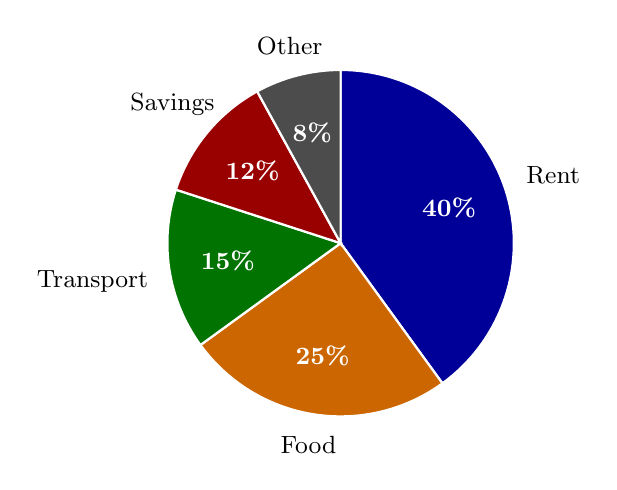
\begin{tikzpicture}[font=\small]
  % Each slice runs clockwise from 12 o'clock; \a and \b are the running totals before and after it, in percent.
  \foreach \p/\name/\c [remember=\b as \a (initially 0), evaluate=\p as \b using \a+\p] in
    {40/Rent/blue!60!black, 25/Food/orange!80!black, 15/Transport/green!45!black, 12/Savings/red!60!black, 8/Other/gray!60!black} {
    \fill[\c, draw=white, thick] (0,0) -- (90-3.6*\a:2.2) arc[start angle=90-3.6*\a, end angle=90-3.6*\b, radius=2.2] -- cycle;
    \pgfmathsetmacro\mid{90 - 1.8*(\a + \b)}
    \node[white, font=\small\bfseries] at (\mid:1.45) {\p\%};
    \node[anchor=\mid+180] at (\mid:2.35) {\name};
  }
\end{tikzpicture}
